
\section{Inbetriebnahme eines Osmocom Systems}
Für Inbetriebnahme des GSM Netzes waren einige Vorinstallationen sowie das Einrichten von Ubuntu 16.04.3 nötig. Im Folgenden wird das Vorgehen zur Einrichtung des Systems sowie die Inbetriebnahme des GSM Netzes beschrieben.

\subsection{Vorinstallationen}
Dieses Kapitel behandelt die für die Installation und Inbetriebnahme notwendigen Softwarevoraussetzungen.

\subsubsection{Ubuntu 16.04.3}\label{ubuntu}
Zunächst wurde wie bei der Installation von Osmocom das Betriebssystem Ubuntu 16.04.3 auf einem Labor-Rechner installiert und eingerichtet. Zusätzlich wurden alle Programme und Pakete mit den folgenden Befehlen aktualisiert.
\begin{lstlisting}
sudo apt-get update
sudo apt-get upgrade
\end{lstlisting}
\subsubsection{Git}
Da die Open-Source Projekte von OsmocomBB auf Git-Repositories liegen, wurde zunächst Git eingerichtet. Zur Versionskontrolle und Verwaltung des Codes wurde außerdem ein Team-eigenes Git Repository angelegt.

\begin{lstlisting}
sudo apt-get install git
\end{lstlisting}

\subsubsection{Softwarevoraussetzungen}
Osmocom empfiehlt zunächst die Einrichtung von einigen Bibliotheken und sonstigen, nötigen Abhängigkeiten als Voraussetzung für die Inbetriebnahme der GSM Komponenten. Diese wurden mittels Paketmanagers wie folgt installiert.

\begin{lstlisting}
sudo apt-get install libpcsclite-dev libtalloc-dev libortp-dev libsctp-dev 
libmnl-dev libdbi-dev libdbd-sqlite3 libsqlite3-dev sqlite3 libc-ares-dev 
libdbi0-dev libdbd-sqlite3 build-essentials libtool autoconf automake pkg-config 
libsqlite3-tcl sqlite-autoconf sqlite-autoconfg
\end{lstlisting}

Die die Fehler bezüglich Bumpversion nicht behoben werden konnten, wurden sie ignoriert. Dies zog keinerlei Konsequenzen hinsichtlich der Inbetriebnahme der GSM Komponenten nach sich.

Zusätzlich bedarf es der separaten Installation der Software Bibliotheken libosmo-abis, libosmocore und libosmo-netif. Diese wurden von den entsprechenden Git Repositories heruntergeladen und nach analogem Vorgehen installiert.

\begin{lstlisting}
git clone git://git.osmocom.org/<lib-source>
cd <lib-source>
autoreconf -fi
./configure
make
make install
sudo ldconfig
\end{lstlisting}

Trotz der sorgfältigen Installation einiger Softwarevoraussetzungen traten zusätzliche Abhängigkeiten bei der Installation einzelner GSM Komponenten auf, welche in \ref{GSM_Komp_Osmocom} beschrieben sind.

\subsubsection{Aktivierung der Verbindung zum USRP2}\label{usrp2_connect}
Vor Installation des Treibers sollte zunächst die Netzwerkschnittstelle aktiviert werden. Die Default IP-Adresse des Ettus USRP2 ist 192.168.10.2. Dafür mussten wir zuerst erfahren, welche Bezeichnung die für den Ettus USRP2 verwendete Schnittstelle nutzt.
\begin{lstlisting}
sudo ifconfig
\end{lstlisting}

Daraufhin konnten wir die IP-Adresse der Schnittstelle am PC so setzen, dass es möglich sein sollte mit dem Ettus USRP2 zu kommunizieren.
\begin{lstlisting}
sudo ifconfig enp0s25 192.168.10.3
ping 192.168.10.2
\end{lstlisting}

Allerdings war zunächst keine Kommunikation mit dem USRP2 möglich, deshalb versuchten wir das Gerät zu finden, indem wir den kompletten IP-Bereich des Netzwerks anpingten sowie die automatische Suchfunktion von UHD-Geräten nutzten.
\begin{lstlisting}
nmap -sP 192.168.10.0/24 | grep -oE '([[:digit:]]{1,3}\.){3}[[:digit:]]{1,3}'
uhd_find_devices
\end{lstlisting}

Nachdem auch diese beiden Befehle zu keinem Erfolg führten und das Gerät auch in anderen IP-Netzbereichen nicht gefunden werden konnte, brachten wir den N210 in den Safe-Mode, in welchem es immer die IP-Adresse 192.168.10.2 besitzt. Dafür mussten wir den N210 aufschrauben und den Safe-Mode Knopf (S2) im Inneren drücken und bis zum erfolgreichen Neustart gedrückt halten. Nun konnten wir das Image des N210 aktualisieren und gleichzeitig die IP-Adresse außerhalb des Safe-Modes auf 192.168.10.2 setzen.
\begin{lstlisting}
uhd_image_loader --args="type=usrp2,addr=192.168.10.2, reset"
sudo /usr/lib/uhd/utils/usrp2_recovery.py --ifc=enp0s25 --new-ip=192.168.10.2
\end{lstlisting}

Die automatische Suchfunktion zeigte nun endlich auch im normalen Modus eine Verbindung.
\begin{lstlisting}
uhd_find_devices

linux; GNU C++ version 5.3.1 20151219; Boost_105800; UHD_003.009.002-0-unknown

--------------------------------------------------
-- UHD Device 0
--------------------------------------------------
Device Address:
    type: usrp2
    addr: 192.168.10.2
    name: 
    serial: F449BF
\end{lstlisting}

\subsection{Installation einzelner GSM Komponenten}\label{GSM_Komp_Osmocom}
OsmocomBB hält detaillierte Beschreibungen zur Installation der GSM Komponenten bereit, welche zur Inbetriebnahme des in Rahmen dieser Arbeit verwendeten GSM Netzes herangezogen wurden. Im Folgenden wird die Installation und Einrichtung der GSM Komponenten genauer erläutert. 

\subsubsection{OsmoTRX}
Zur Kommunikation mit der Basisstation ist der osmoTRX Transceiver nötig. Osmocom bietet diesen - meist wie die anderen Komponenten - im Git Repository an. Die Installation des Transceiver erforderte die Bibliotheken \textit{$libusb-1.0-0-dev$, $uhd-host$, $libboost-dev$} und \textit{$libuhd-dev$}. Diese bieten die Suchfunktion \textit{uhd\_find\_devices}. Dadurch lässt sich testen, ob die Basisstation gefunden wird. Mittels \textit{osmo-trx} lässt sich der Transceiver nach der Installation starten.

\begin{lstlisting}
git clone git://git.osmocom.org/osmo-trx
cd osmo-trx/
autoreconf -i
./configure
sudo make -j8
sudo make install
osmo-trx	
\end{lstlisting}

\begin{figure}[h] %t=top b=bottom h=here p =eigene page
\centering
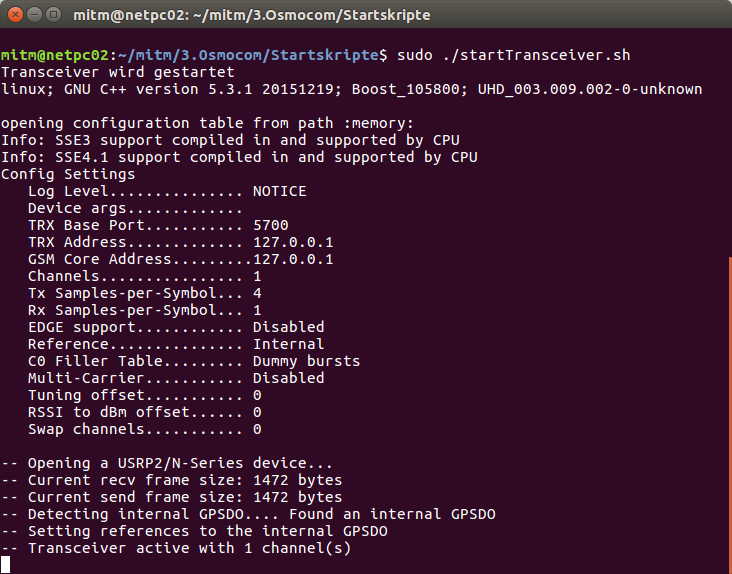
\includegraphics[width=15cm]{includes/Start_Transceiver}
\caption{Ansicht der Konsole nach dem Start des Transceivers}
\label{fig:Transceiver}
\end{figure}

Zur Behebung der Warnung, die in Abbildung \ref{fig:UHDWarnung} zu sehen ist, wurde die Priorität in der Datei /etc/security/limits.conf gesetzt.

\begin{lstlisting}
@usrp   -  rtprio  50
\end{lstlisting}

\begin{figure}[h] %t=top b=bottom h=here p =eigene page
\centering
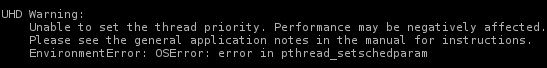
\includegraphics[width=15cm]{includes/uhd_usrp_warnung}
\caption{Fehlermeldung bezüglich der Thread Priorität in osmoTRX}
\label{fig:UHDWarnung}
\end{figure}

\subsubsection{OsmoBTS}
Die Installation von OsmoBTS erfolgte analog zur Einrichtung der anderen Osmocom Komponenten.

\begin{lstlisting}
git clone git://git.osmocom.org/osmo-bts.git
autoreconf -fi
cd osmo-bts
./configure --enable-trx
sudo make -j8
sudo make install
\end{lstlisting}

Zur Konfiguration wurden zunächst die Pfade der folgenden Variablen angepasst.

\begin{lstlisting}
PATH="/usr/local/sbin:/usr/local/bin:/usr/sbin:/usr/bin:/sbin:/bin:/usr/games:/usr/local/games"
PKG_CONFIG_PATH="/home/netpc06/libosmo-abis/"
LIBOSMOTRAU_CFLAGS="/home/netpc06/libosmo-abis/"
LIBOSMOTRAU_LIBS="/home/netpc06/libosmo-abis/"
\end{lstlisting}

Weiterhin erforderte die Konfiguration von OsmoBTS Änderungen an der Datei osmo-bts.cfg (siehe Anhang \ref{Osmo-bts.cfg}). Es wurde die Option \textit{band} auf PCS1900 gesetzt, welche dem lizenzierten Frequenzband entspricht. Des Weiteren wurde    die Signalstärke durch Angabe des \textit{osmotrx rx-gain} auf 1 gesetzt. Eine letzte Änderung wurde an der lokalen und remote IP vorgenommen, welche auf 127.0.0.1 gesetzt wurde. \\

Die Konfigurationsdatei wurde unter dem Pfad \textit{/home/netpc06/osmo-bts/src/osmo-bts-trx} abgelegt. 

\subsubsection{OsmoNitb unter OpenBSC}
Weiterhin wurde OpenBSC installiert. Dazu wurde die Bibliothek \textit{libssl-dev} (eigentlich unter \textit{libcrypto} bekannt) vorausgesetzt.

\begin{lstlisting}
sudo apt-get install libssl-dev
git clone git://git.osmocom.org/openbsc
cd openbsc/
cd openbsc/openbsc/
autoreconf -i
./configure 
sudo make -j8
sudo make install
\end{lstlisting}

Zur Konfiguration von OpenBSC wurde - analog zu OsmoBTS - eine Beispieldatei wie folgt angepasst (siehe Anhang \ref{Openbsc.cfg}). \textit{short name} und \textit{long name} beschreiben den Name des Netzwerks und wurden umbenannt. Die Option \textit{auth policy} wurde auf \textit{accept-all} gesetzt, um alle Anfrage zur Registrierung im Netz zuzulassen. Andernfalls muss die IMSI der jeweiligen Mobilfunkstation (MS) in der Datenbank des Home Location Registers (HLR) hinterlegt sein. Da der erlaubte Frequenzbereich 1909,0/1989,0 MHz beträgt, wurde die Option \textit{band} auf \textit{PCS1900} gesetzt. Weiterhin wurde die \textit{ipa.unit-id} an die der OsmoBTS angepasst (1901 0). Eine letzte Änderung wurde an der sogenannten Absolute Radio Frequency Channel Number (ARFCN) vorgenommen, die durch die Option \textit{arfcn} angegeben wird. Dieser ergibt sich wie folgt:

\begin{equation}
ARFCN = Offset + \frac{f_{up} - f_{UplinkStart}}{f_{bandbreite}}
\end{equation}

Der oben genannte Frequenzbereich lässt sich auf ein Netzwerk vom Typ PCS1900 zurückführen. Als \textit{Offset} wurde ein Wert von 512 gewählt, der für diesen Frequenzbereich üblich ist. $f_{up}$ wurde auf einen Wert von 1850,2 MHz gesetzt, da dieser der Startwert des Uplinks für das PCS1900 ist. In der Frequenzzuteilung der Bundesnetzagentur wurde eine Bandbreite von 0,2 MHz angegeben. Unter Verwendung dieser Werte ergibt sich ein ARFCN von 806.\\

Nach Änderung der Konfigurationsdatei openbsc.cfg wurde diese unter dem Pfad \textit{/home/netpc06
/openbsc/openbsc/src/osmo-nitb} abgelegt.

\subsection{Starten des Systems}
Nach Installation aller Komponenten wurde das System gestartet. Dabei wurden als Optionen die Pfade der Konfigurationsdateien angeben. Da OsmoBTS den Transceiver fordert, musste dieser als erste Instanz gestartet werden. Die Reihenfolge der weiteren Komponenten spielt keine Rolle. 

\begin{lstlisting}
// Transceiver starten
cd /home/netpc06/osmo-trx
sudo osmo-trx -f
\end{lstlisting}

Als Option beim Start von Osmo-Nitb wurden sowohl der Pfad der Konfigurationsdatei als auch der der HRL Datenbank angegeben.
\begin{lstlisting}
cd /home/netpc06/openbsc/openbsc/src/osmo-nitb
osmo-nitb -c /home/netpc06/openbsc/openbsc/src/osmo-nitb/openbsc.cfg -l /home/netpc06/openbsc/openbsc/src/osmo-nitb/hlr.sqlite3 -P -C --debug=DRLL:DCC:DMM:DRR:DRSL:DNM
\end{lstlisting}

\begin{figure}[h] %t=top b=bottom h=here p =eigene page
\centering
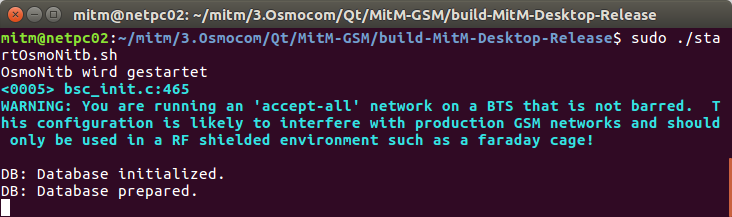
\includegraphics[width=15cm]{includes/Start_OsmoNitb}
\caption{Ansicht der Konsole nach dem Start der OsmoNitb}
\label{fig:OsmoNitb}
\end{figure}

\newpage
OsmoBTS wurde wie folgt gestartet.

\begin{lstlisting}
cd /home/netpc06/osmo-bts/src/osmo-bts-trx
sudo osmo-bts-trx -c osmo-bts.cfg
\end{lstlisting}

\begin{figure}[h] %t=top b=bottom h=here p =eigene page
\centering
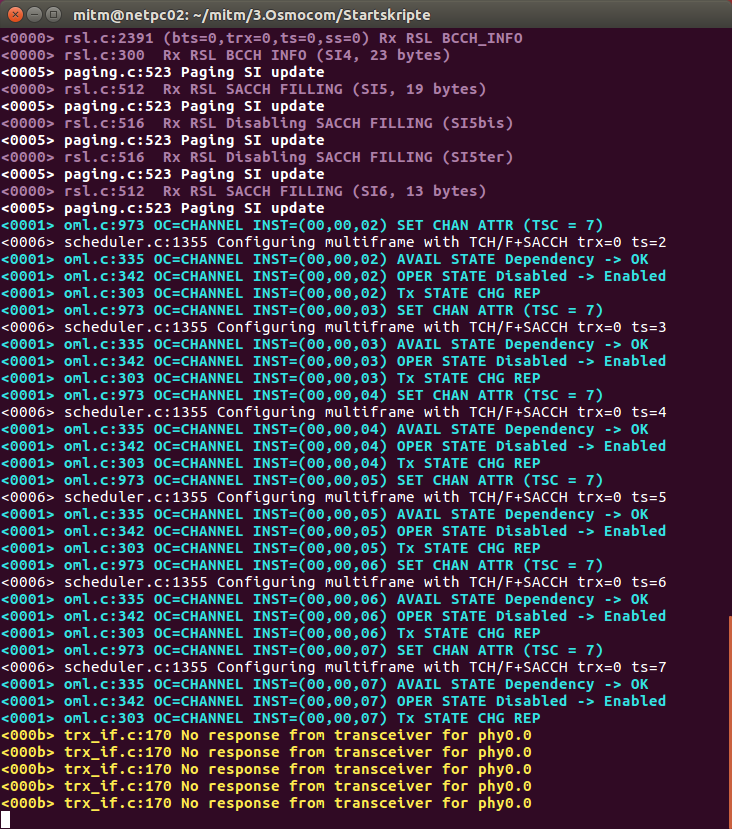
\includegraphics[width=15cm]{includes/Start_OsmoBTS}
\caption{Ansicht der Konsole nach dem Start der OsmoBTS}
\label{fig:OsmoBTS}
\end{figure}


\subsection{Installation weiterer Komponenten}
Neben den Komponenten zur Inbetrienahme des GSM Netzes wurden außerdem weitere Installationen vorgenommen. Diese waren zur Umsetzung des Projektziels notwendig.

\subsubsection{Osmo-sip-Connector}
Zur Konvertierung von .wav-Dateien werden sowohl RTP als auch SIP Pakete benötigt. Um neben RTP und UDP Paketen auch SIP Pakete abfangen zu können, wurde der Osmo-sip-Connector wie folgt installiert.

\begin{lstlisting}
git clone git://git.osmocom.org/osmo-sip-connector.git
cd osmo-sip-connector/
autoreconf -fi
./configure
make
sudo make install
\end{lstlisting} 

Nach erfolgreicher Installation wurde der Osmo-sip-connectors mit Angabe der Konfigurationsdatei gestartet.

\begin{lstlisting}
osmo-sip-connector -c ./osmo-sip-connector.cfg
\end{lstlisting} 

\begin{figure}[h] %t=top b=bottom h=here p =eigene page
\centering
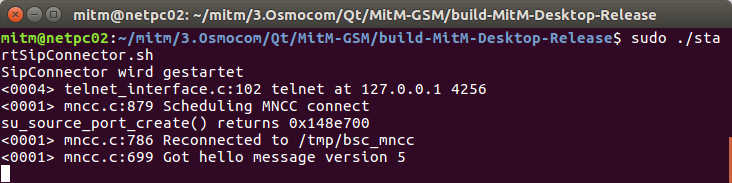
\includegraphics[width=15cm]{includes/Start_SipConnector}
\caption{Ansicht der Konsole nach dem Start des Osmo-sip-connectors}
\label{fig:Asterisk}
\end{figure}
 
\subsubsection{Asterisk}
Den Aufbau von Gesprächen sowie deren Vermittlung wurde in dieser Arbeit der PBX Asterisk verwendet. Dieser wurde über den Paketmanager installiert. Die Einrichtung erforderte die Installation der Bibliothek \textit{libsofia-sip-ua-glib-dev}.

\begin{lstlisting}
sudo apt-get install asterisk
\end{lstlisting}

Nach der Installation startet Asterisk selbständig. Da mehrmals Änderungen an den Konfigurationsdateien von Asterisk vorgenommen wurden, wurde Asterisk mehrmals neu gestartet.

\begin{lstlisting}
core restart gracefully
sudo asterisk -r
\end{lstlisting}

Nach mehreren Fehlschlägen bezüglich der Installation von Asterisk und folglichem Neuaufsetzen des gesamten Systems inklusive des Betriebssystems wurde Asterisk als erste Komponente vor der GSM Installation eingerichtet. Es stellte sich heraus, dass dieses Vorgehen zu einer erfolgreichen Installation von Asterisk und Inbetriebnahme des GSM Netzes führte.

\begin{figure}[h] %t=top b=bottom h=here p =eigene page
\centering
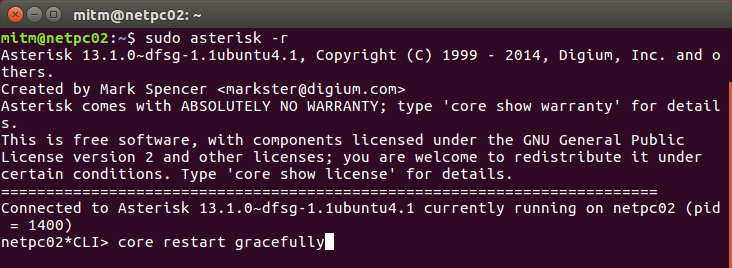
\includegraphics[width=15cm]{includes/Asterisk}
\caption{Ansicht der Konsole nach Verbindung mit Asterisk}
\label{fig:Asterisk}
\end{figure}